\documentclass[border=5pt]{standalone}
\usepackage{tikz}
\usepackage{amsmath}
\usetikzlibrary{arrows.meta, positioning, shapes.geometric, calc}

\begin{document}
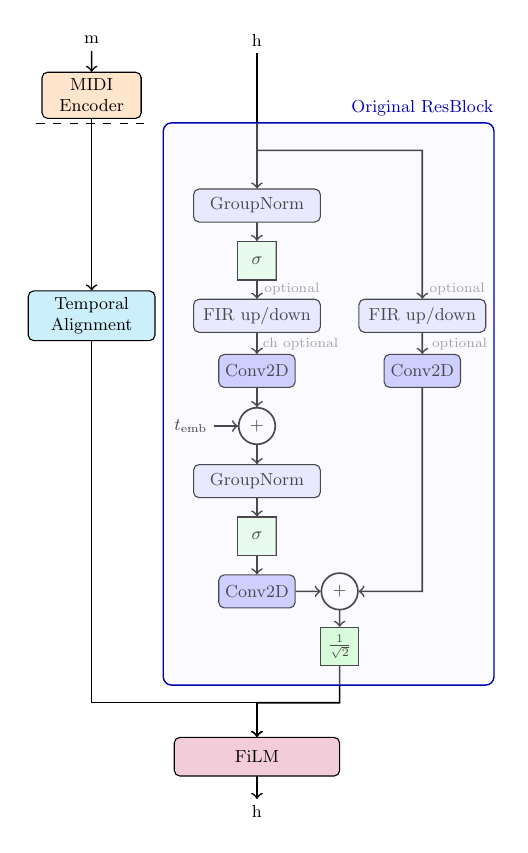
\begin{tikzpicture}[
  scale=0.7, transform shape,
  font=\small,
  box/.style = {draw, rounded corners=2pt, minimum width=23mm,
                minimum height=6mm, align=center},
  smallbox/.style = {draw, rounded corners=2pt, minimum width=18mm,
                     minimum height=6mm, align=center},
  convbox/.style = {draw, rounded corners=2pt, minimum width=10mm,
                    minimum height=6mm, align=center},
  filmbox/.style = {draw, rounded corners=2pt, minimum width=30mm,
                    minimum height=7mm, align=center},
  cubebox/.style = {draw, minimum width=18mm, minimum height=7mm, 
                    align=center, fill=gray!10, rounded corners=2pt,
                    path picture={
                      \draw[fill=gray!20] 
                        (path picture bounding box.north east) -- ++(2mm,2mm) -- ++(0,-7mm) -- 
                        (path picture bounding box.south east) -- cycle;
                      \draw[fill=gray!15] 
                        (path picture bounding box.north east) -- ++(2mm,2mm) -- ++(-18mm,0) -- 
                        (path picture bounding box.north west) -- cycle;
                    }},
  greencubebox/.style = {draw, minimum width=7mm, minimum height=7mm, 
                    align=center, fill=green!10,
                    path picture={
                      \draw[fill=green!20] 
                        (path picture bounding box.north east) -- ++(2mm,2mm) -- ++(0,-7mm) -- 
                        (path picture bounding box.south east) -- cycle;
                      \draw[fill=green!15] 
                        (path picture bounding box.north east) -- ++(2mm,2mm) -- ++(-18mm,0) -- 
                        (path picture bounding box.north west) -- cycle;
                    }},
  arrow/.style = {->, >=Classical TikZ Rightarrow, semithick}
]

% Inputs
\node (h_input) at (0,20mm) {h};
\node (midi_input) at (-30mm,20mm) {m};

% MIDI path (outside box)
\node[cubebox, fill=orange!20] (midi_encoder) at (-30mm,10mm) {MIDI\\Encoder};

% Start of boxed content
\node[box, fill=cyan!20] (temporal_align) at (-30mm,-30mm) {Temporal\\Alignment};

% H path 1: h -> GroupNorm -> SiLU
\node[box, fill=blue!10] (groupnorm) at (0,-10mm) {GroupNorm};
\node[greencubebox] (silu) at (0,-20mm) {$\sigma$};

% Continue from SiLU
\node[box, fill=blue!10] (fir2) at (0,-30mm) {FIR up/down};
\node[anchor=south east, font=\scriptsize, text=gray] at ([xshift=1mm, yshift=-0.5mm]fir2.north east) {optional};
\node[convbox, fill=blue!25] (conv2d2) at (0,-40mm) {Conv2D};
\node[anchor=south east, font=\scriptsize, text=gray] at ([xshift=9mm, yshift=-0.5mm]conv2d2.north east) {ch optional};

% Addition with t_emb
\node[circle, draw, minimum size=6mm, fill=white, semithick] (plus) at (0,-50mm) {$+$};
\node (t_emb) at (-12mm,-50mm) {$t_{\text{emb}}$};

\node[box, fill=blue!10] (groupnorm2) at (0,-60mm) {GroupNorm};
\node[greencubebox] (silu2) at (0,-70mm) {$\sigma$};
\node[convbox, fill=blue!25] (conv2d3) at (0,-80mm) {Conv2D};

% H path 2: h -> FIR up/down -> Conv2D
\node[box, fill=blue!10] (fir) at (30mm,-30mm) {FIR up/down};
\node[anchor=south east, font=\scriptsize, text=gray] at ([xshift=1mm, yshift=-0.5mm]fir.north east) {optional};
\node[convbox, fill=blue!25] (conv2d) at (30mm,-40mm) {Conv2D};
\node[anchor=south east, font=\scriptsize, text=gray] at ([xshift=6mm, yshift=-0.5mm]conv2d.north east) {optional};

% Addition of two Conv2D outputs
\node[circle, draw, minimum size=6mm, fill=white, semithick] (plus2) at (15mm,-80mm) {$+$};

% Multiplication by 1/sqrt(2)
\node[greencubebox, fill=green!20] (scale_factor) at (15mm,-90mm) {$\frac{1}{\sqrt{2}}$};

% FiLM at the end
\node[filmbox, fill=purple!20] (film) at (0mm,-110mm) {FiLM};

% Output
\node (output) at (0mm,-120mm) {h};

% Arrows
\draw[arrow] (h_input) -- (groupnorm);
\draw[arrow] (groupnorm) -- (silu);
\draw[arrow] (silu) -- (fir2);
\draw[arrow] (fir2) -- (conv2d2);
\draw[arrow] (conv2d2) -- (plus);
\draw[arrow] (t_emb) -- (plus);
\draw[arrow] (plus) -- (groupnorm2);
\draw[arrow] (groupnorm2) -- (silu2);
\draw[arrow] (silu2) -- (conv2d3);
\draw[arrow] (h_input) |- ++(30mm,-20mm) -- (fir);
\draw[arrow] (fir) -- (conv2d);

% Connect two Conv2D outputs to addition
\draw[arrow] (conv2d3) -- (plus2);
\draw[arrow] (conv2d) -- ++(0,-40mm) -- (plus2);

% Connect addition to multiplication, then combine with temporal alignment at FiLM
\draw[arrow] (plus2) -- (scale_factor);
\draw[arrow] (scale_factor) -- ++(0,-10.2mm) -| (film);
\draw[arrow] (temporal_align.south) |- ++(0,-65.6mm) -| (film);
\draw[arrow] (film) -- (output);

% Draw box around main processing (excluding MIDI encoder)
\draw[blue!70!black, line width=0.5pt, rounded corners=3pt, fill=blue!5, fill opacity=0.3]
  (-17mm,5mm) rectangle (43mm,-97mm);

% Add label on top of the box
\node[anchor=south, font=\small\normalfont, text=blue!70!black] at (30mm,5mm) {Original ResBlock};

% Arrows connecting MIDI path (outside box)
\draw[arrow] (midi_input) -- (midi_encoder);
\draw[arrow] (midi_encoder) -- (temporal_align);

% Horizontal dashed line crossing the MIDI encoder to temporal alignment arrow
\draw[dashed, black!70!black, line width=0.2pt] (-40mm,5mm) -- (-20mm,5mm);

\end{tikzpicture}
\end{document}
